\section{Unified Occlusion Models}
%\section{Occlusion-Aware Association and Localization}
\label{sec:unified}

In this section, we highlight the versatility of our occlusion modeling by demonstrating its unified application to two different problems: associating point tracks with objects and 3D object localization using object and point tracks.

\subsection{Object-Point Association}
\label{sec:association}

Consider the problem of assigning 2D point tracks among several objects (including background), so that the consensus of points can be used draw inferences about the object. In particular given a set of corresponding 2D points $\trackpj{t-1}$ and $\trackpj{t}$ in consecutive frames, object poses $\relp{i}{t}$ and object dimensions $\dimsn{i}$, we wish to associate points with various objects. We call this the association problem. Even if the pose of the object is not immediately available, we propose the use of hypothesized pose of the object as we show in the localization estimation experiments. 

Based on our continuous occlusion model in Section~\ref{sec:setup}, the association probability $\assocP$ of the $j$\textsuperscript{th} point track with $i$\textsuperscript{th} object at depth $\lambda$ can be defined as
\begin{align}
\assocP = \Prefl\Ptrans,
\label{eq:defineassocP}
\end{align}
where $\Prefl$ and $\Ptrans$ are from \eqref{eq:evalPrefl} and \eqref{eq:evalCumulativePtrans} respectively. Note that the fraction $\assocP$ although called association probability does not capture the entire information that we have available for computing association of point tracks to objects. This above fraction is the association probability given the hypothesized parameters of objects in the scene. 

To compute the association probability $\assocP$ between point track $j$ and object $i$, we must use the reprojection error as well. When the association of $i$ and $j$ is correct and the point of reflection is at depth $\lambda$, the reprojection error must be zero \eqref{eq:reprojerror}, otherwise the error becomes a measure of distance from the true solution. The error term can be converted to probability domain by considering the error term as negative log of probability
\begin{align}
  P^{(ij)}_{\text{assoc by reproj}}(\lambda) = \frac{1}{Z}\exp(-\Ereproj(\lambda))
\end{align}

Using both of the above evidence terms we can write the probability of association $P^{(ij)}_{\text{assoc}}$ as follows
\begin{align}
  P^{(ij)}_{\text{assoc}} = \frac{1}{Z'}\int_0^{\infty} \assocP \exp(-\Ereproj(\lambda))d\lambda
  \label{eq:prob-assoc}
\end{align}
Once we have the probability of association $P^{(ij)}_{\text{assoc}}$ we can compute the best possible assignment of object for each point track. The points having very small association probability are assigned to the background,
\begin{align}
  i^*_{j} = \arg \min_{i} \int_0^\infty \assocP \Ereproj(\lambda) d\lambda
\end{align}


In contrast to the principled approach above, a heuristic baseline may simply assign a point to the detection bounding box enclosing it (and background if outside all bounding boxes). For regions where bounding boxes overlap, it may assign point tracks to the object that has smaller mean depth among the competing bounding boxes. As we will demonstrate in experiments, such heuristics are sub-optimal compared to using \eqref{eq:prob-assoc} inspired by our occlusion model.

%For the baseline method, the associations between point tracks and TPs are achieved by using detection bounding boxes, where point tracks within each bounding box are simply assigned to it. For the regions where the bounding boxes overlap, we assign the point tracks to the TP that has smaller mean depth than the competing bounding boxes.



\subsection{3D Object Localization}
\label{sec:localization}

%To show the effectiveness of our method we apply it to the localization problem. We estimate the position, orientation and dimensions of the car with our framework and compute the error in birds eye view domain along the ground plane. To estimate the localization of traffic participants (TPs) in a road scene we use the graphical model approach. We build the graphical model as shown in Fig~\ref{fig:graphmodel} that allows us to factorize the intractable probability distribution into following form

To show the effectiveness of our method we also apply it to the localization problem, where we must jointly solve for association and object poses, while considering occlusions. In road scenes, we estimate the position, orientation and dimensions traffic participants (cars) with our framework and compute the error in birds eye view along the ground plane. We propose a graphical model as shown in Figure \ref{fig:graphmodel} that allows a factorization of the intractable probability distribution into following form
%
\begin{multline}
  -\log{P(\{\state{i}{t}\} | \mathbb{E})} = 
  -Z' 
  \\
  + \sum_{t=s_i}^{e_i}
  \left(
  \sum_{i,j:i\ne j}   
  \WEnergyCol 
   + \WpEnergy{detect}
   + \WpEnergy{track}
\right)
  \\
  + \left(
  \sum_{i=1}^N 
  \WEnergy{lane}
  + \WEnergy{dyn}
  + \WEnergy{size}
\right)
  \enspace.
\end{multline}
%
Next, we explain the important energies used in our graphical model.


\begin{figure}
  \centering
  \begin{tabular}{c}
    \newcommand{\imagewidth}{7cm}
    ../../CVPR/Source/scenelayoutoverlayCity0961.tex \\
    \usetikzlibrary{trees,shadows}
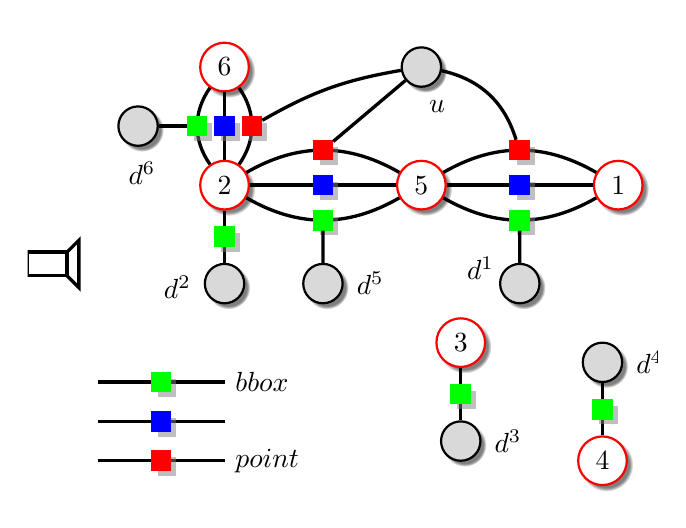
\begin{tikzpicture}[grow cyclic, line width=1.2pt,
    variablenode/.style={circle,circular drop shadow,draw=red,fill=white,thick,minimum width=0.5cm},
   bboxfactor/.style={rectangle,drop shadow,draw=green,fill=green,thick,minimum width=0.2cm},
    collfactor/.style={rectangle,drop shadow,draw=blue,fill=blue,thick,minimum width=0.2cm},
    trackfactor/.style={rectangle,drop shadow,draw=red,fill=red,thick,minimum width=0.2cm},
  obs/.style={fill=gray!30,draw=black},
  prevf/.style={draw=green!20,text=gray},
  prevobsv/.style={draw=gray!10,fill=gray!1,text=gray},
  prevv/.style={draw=red!20,text=gray}
]
  \path[use as bounding box,clip] (-2.5, -5.5) rectangle (5.5,0.5);
  \draw (-2.5,-2.65) rectangle +(0.5,0.3);
  \draw (-2.0,-2.35) -- ++(0.15, 0.15) -- ++(0, -0.6) -- (-2.0, -2.65);
\path
     (0, 0)  node [variablenode] (x6) {6}
++(0, -1.5) node [variablenode] (x2) {2}
++(2.5, 0)  node [variablenode] (x5) {5}
+ (0, 1.5)  node [variablenode,obs] (u) {}
+(.2,1.0)  node {$u$}
+ (.5, -2)   node [variablenode] (x3) {3}
+ (2.3, -3.5)   node [variablenode] (x4) {4}
+(2.5, 0)  node [variablenode] (x1) {1}
;

% Factors between nodes 6 and 2
\draw (x6) edge [bend right=35] node [bboxfactor] (f26) {} (x2);
\path (f26) +(-0.75,0) node [variablenode,obs] (d6) {} 
                        +(-.7,-.6)  node {$d^6$};
\draw (f26) edge (d6);
\draw (x6) edge [bend left=35] node [trackfactor] (ft26) {} (x2);
\draw (ft26) edge [bend left=10] (u);
\draw (x6) edge node [collfactor] {} (x2);

% Factors for node 2
\path (x2) +(0,-1.25) node [variablenode,obs] (d2) {} 
                        +(-.6,-1.3)  node {$d^2$};
\draw (x2) edge node [bboxfactor] {} (d2);

% Factors between nodes 2 and 5
\draw (x2) edge [bend right] node [bboxfactor] (f25) {} (x5);
\draw (x2) edge [bend left] node [trackfactor] (ft25) {} (x5);
\draw (x2) edge [] node [collfactor] {} (x5);
\draw (ft25) edge (u);
\path (x5) ++(-1.25,-1.25) node [variablenode,obs] (d5) {} 
                        +(.6,0)  node {$d^5$};
\draw (f25) edge (d5);

% Factors between nodes 5 and 1
\draw (x5) edge [bend right] node [bboxfactor] (f51) {} (x1);
\draw (x5) edge [bend left] node [trackfactor] (ft51) {} (x1);
\draw (x5) edge [] node [collfactor] {} (x1);
\draw (ft51) edge [bend right] (u);
\path (x1) ++(-1.25,-1.25) node [variablenode,obs] (d1) {} 
                        +(-.5,0.2)  node {$d^1$};
\draw (f51) edge (d1);

% Factors for node 3
\path (x3) ++(0,-1.25) node [variablenode,obs] (d3) {} 
                        +(.6,0)  node {$d^3$};
\draw (x3) edge node [bboxfactor] {} (d3);

% Factors for node 4
\path (x4) ++(0,1.25) node [variablenode,obs] (d4) {} 
                        +(.6,0)  node {$d^4$};
\draw (x4) edge node [bboxfactor] {} (d4);

% Legend
\path (-1.75,-4.0) node (l1s) {} (-0, -4.0) node [anchor=west] (l1e) {$\Energy{bbox}$};
\draw (l1s) edge node [bboxfactor] {} (l1e);
\path (-1.75,-4.5) node (l2s) {} (0, -4.5) node [anchor=west] (l2e) {$\EnergyCol$};
\draw (l2s) edge node [collfactor] {} (l2e);
\path (-1.75,-5.0) node (l3s) {} (0, -5.0) node [anchor=west] (l3e) {$\Energy{point}$};
\draw (l3s) edge node [trackfactor] {} (l3e);

\end{tikzpicture}

  \end{tabular}
  \caption{\small (Top) A sample road scene with occlusions, where the unknowns of each car are modeled as random variables. (Bottom) Graphical model for a single frame. The six numbered nodes represent the unknown state variables of each car. The shaded nodes in the graphical model are observed variables (detection bounding boxes and point tracks), while the colored squares represent various energies that capture object-object interactions.}
  \label{fig:graphmodel}
\end{figure}



\subsubsection{Continuous point tracks energy with occlusion}
\label{sec:totalContPtTracksEnergy}

Let the pose of object $i$ at time $t$ be $\relp{i}{t}$. We denote $\projectionOf{.}$ and $\invProjectionOftm{.}$ for the forward and inverse projection functions that project a 3D point to the camera image and vice versa. Then, the reprojection error for the $j$\textsuperscript{th} 2D point, $\trackp{t}$, with hypothesized depth $\lambda$, is given by
\begin{equation}
\Ereproj(\lambda) = \left\|\trackpj{t} - \projectionOf{\invProjectionOftm{\trackpj{t-1}, \lambda}}\right\|^2.
\label{eq:reprojerror}
\end{equation}
Note that inverse projection $\invProjectionOf{.}$ depends on both the 2D point $\trackp{t}$ and the unknown depth $\lambda$. Also note that the inverse projection is dependent on object pose at time $t-1$ while the forward projection depends on pose at time $t$, which can be different.

For an object $i$, let $\{ \Omega (t) \}_i$ be the poses of all occluding objects at time $t$ (inclusive of object $i$) and $ \{ \bB \}_i$ be their dimensions. Then, we model the continuous point tracks energy with explicit occlusion reasoning as the expected reprojection error over the association probability:
\begin{multline}
  %\!\!\!\! \Energy{track}(\relp{i}{t}, \relp{i}{t-1}, \dimsn{i}, \{ \Omega (t) \}_i, \{ \Omega (t-1) \}_i, \{ \bB \}_i ) 
  %\Energy{track}(\{ \relp{i}{t} \}_i, \{ \relp{i}{t-1} \}_i, \{\dimsn{i}\}_i ) = 
  \Energy{track}(\{ \Omega (t) \}_i, \{ \Omega (t-1) \}_i, \{ \bB \}_i )
  \\
    = \sum_{i=1}^{N} 
    %\sum_{t = s_i}^{e_i}
    \sum_{j = 1}^{M}
    \int_1^\infty \assocP\Ereproj(\lambda) d\lambda
\end{multline}
where $\assocP$ is the association probability of the $j$\textsuperscript{th} point with the $i$\textsuperscript{th} object at depth $\lambda$, given by \eqref{eq:defineassocP}.

%\begin{align}
%  \assocP &= \Prefl\Ptrans\\
%  \Ereproj(\lambda) &= \left\|\trackpj{t} - \projectionOf{\invProjectionOftm{\trackpj{t-1}, \lambda}}\right\|^2 .
%  \label{eq:reprojerror}
%\end{align}

%The $\projectionOf{.}$ and $\invProjectionOftm{.}$ denote the projection and inverse projection functions that project 3D point to camera image and vice versa. Note that inverse projection $\invProjectionOf{.}$ depend on both the point $\trackp{t}$ and the unknown depth $\lambda$. Also note that the inverse projection is dependent on TP pose at time $t-1$ while the projection depends on pose at time $t$ which can be different.

\subsubsection{Continuous bounding box energy with occlusion}

Object detection is usually followed by non-maximal suppression that results in discarding similar bounding boxes. When we are jointly optimizing detections with other cues, it is not usually desirable to go with a single bounding box. To retain the entire detection output while maintaining the continuous form of our energies, we approximate the distribution of detection scores with a multi-modal sum of Gaussians-like logistic functions. In particular, let $\bb{i}$ be a detection bounding box for object $i$, parameterized as a 4D vector $[\minx, \miny, \maxx, \maxy]^\top$. We fit a parametric function to the detection scores, of the form
\begin{equation}
S(\bb{i}) = \sum_k A_k \exp \left( -\bepsilon_k^{(i)}(t)^\top \Lambda_k^{'-1} \bepsilon_k^{(i)}(t) \right)
\end{equation}
where $A_k$ is an amplitude and $\bepsilon_k^{(i)}(t) = \bb{i}-\mu^{(k)}_d$, with $\mu^{(k)}_d$ the mean and $\Lambda_k$ the covariance.
%% %
%% \begin{multline}
%%   S(\bb{i}) = \\
%%   \sum_k A_k \exp(-(\bb{i}-\mu^{(d)}_k)^\top \Sigma^{(d)-1}_k
%%   (\bb{i}-\mu^{(d)}_k))
%% \end{multline}
%% %
%% to detection scores, by 
We use a non-linear solver to minimize the above, with initialization from non-maximal suppressed outputs. The optimization is constrained by the symmetry and positive definiteness of $\Lambda_k^{-1}$, $\maxx \ge \minx$ and $\maxy \ge \miny$.
%Here $\mu^{(d)}_j$ is one of the $k$ modes as a 4D vector representing a single bounding box as $[\minx, \miny, \maxx, \maxy]^\top$. The optimization is constrained with symmetry and positive definiteness of $\Sigma^{(d)-1}_k$, $\maxx \ge \minx$ and $\maxy \ge \miny$.

\paragraph{Detection scores with occlusion reasoning} 
\def\u{\mathbf{u}}
With our model of $\Ptrans$ described in Section \ref{sec:ptransmission}, we can
compute the probability of a point $\u$ in the image to be occluded assuming
the point is on object $i$ with mean depth $\meandepth{i}$ as
\begin{align}
  O_{i}(\u, \meandepth{i}) = 1 - \Ptransmission(\meandepth{i}, \u) \enspace .
\end{align}

If a portion of our proposed detection bounding box is known to be
occluded, then we would like to decrease the confidence in the detection score
about the localization of that end of the object. Assuming that the occlusion
is often on the boundary of detection bounding boxes, we want to decrease our
confidence on the mean detection boundaries around the occluded boundaries.
To re-model our detection scores scaled by continuous occlusion we sample
$O_{i}(\mathbf{u}, \meandepth{i})$ at the hypothesized detection boundaries from
GMM $S(.)$ and we augment the detection boundary covariance matrix by
$\mathcal{P}_{i} = \rho_{i}\rho_{i}^\top$ where $\rho_{i} = O_{i}(\mathbf{u},
\meandepth{i})$. The new covariance matrix in detection score is given by 
  $\Lambda'_k = \mathcal{P}_{i} + \Lambda_k$ for all $k$.
The detection scores GMM with occlusion is given by replacing the covariance
matrix
%
\begin{multline}
S'(\bb{i}) = \sum_k A_k \exp \left( -\bepsilon_k^{(i)}(t)^\top \Lambda_k^{'-1} \bepsilon_k^{(i)}(t) \right)
\end{multline}

The energy of detection scores is simply take to be the inverse of the detection score.
\begin{align}
  \Energy{detect}(\{ \relp{i}{t} \}_i, \{ \relp{i}{t-1} \}_i, \{\dimsn{i}\}_i ) = \frac{1}{S'(\bb{i})}
\end{align}

For object detections we use object detector by \cite{Felzenszwalb_etal_2010}
which is detector by parts model and we use eight parts to train the car model 
on half of the KITTI dataset \cite{geiger2013vision}. The trained modeled is 
used to get detections for the other half of the dataset and vice versa. 

\subsubsection{Other energies}
Other energies we use are described in detail in the supplementary material. We briefly describe them here:
\begin{description}
  \item[Lane energy ($\Energy{lane}$)] This energy term constrains the
    orientation of traffic participants to be parallel to the nearest detected
    lane. The lanes are either detected visually or obtained from GPS and Map 
    information.
  \item[Transition probability ($\Energy{dyn}$)] We use these energies to
    constrain the motion of cars to be smooth in linear motion and rotation
    motion. We also constrain cars to move in the direction of heading.
  \item[Size prior ($\EnergySize$)] We use size prior of cars by using the mean
    of cars over the KITTI dataset.
\end{description}

\subsection{Metropolis Hastings Inference}
We use Metropolis Hastings' methods \cite{mackay1998introduction} for graphical model inference. Since we are
optimizing over continuous random variables, we use Gaussian distribution as
the proposal distribution. We choose Metropolis Hastings inference over
block-coordinate descent which turns out to be slower than Metropolis Hastings
in our experiments. Please refer to the supplementary material for the
comparison of inference methods.

%% \begin{figure}
%%   \centering
%%   \newcommand{\imagewidth}{\columnwidth}
%%   ../../CVPR/Source/scenelayoutoverlayCity0961.tex
%%   \caption{A sample road scene with the unknowns of each car modeled as random variables. 
%%   The relating energies are shown in Figure~\ref{fig:graphmodel}}
%% \end{figure}
%% \begin{figure}
%%     \usetikzlibrary{trees,shadows}
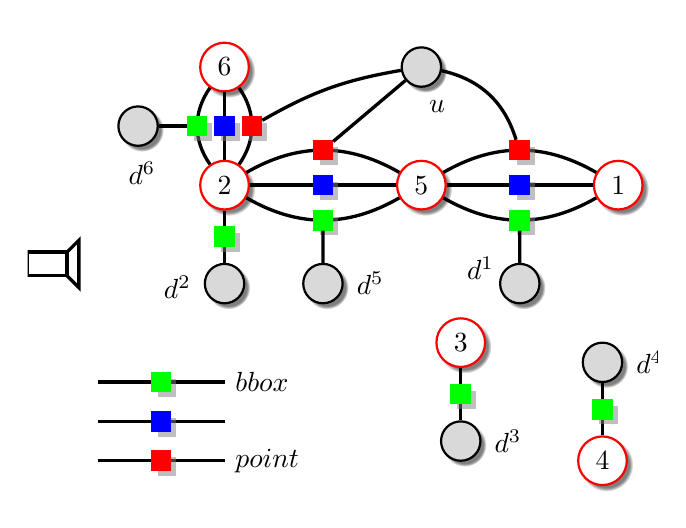
\begin{tikzpicture}[grow cyclic, line width=1.2pt,
    variablenode/.style={circle,circular drop shadow,draw=red,fill=white,thick,minimum width=0.5cm},
   bboxfactor/.style={rectangle,drop shadow,draw=green,fill=green,thick,minimum width=0.2cm},
    collfactor/.style={rectangle,drop shadow,draw=blue,fill=blue,thick,minimum width=0.2cm},
    trackfactor/.style={rectangle,drop shadow,draw=red,fill=red,thick,minimum width=0.2cm},
  obs/.style={fill=gray!30,draw=black},
  prevf/.style={draw=green!20,text=gray},
  prevobsv/.style={draw=gray!10,fill=gray!1,text=gray},
  prevv/.style={draw=red!20,text=gray}
]
  \path[use as bounding box,clip] (-2.5, -5.5) rectangle (5.5,0.5);
  \draw (-2.5,-2.65) rectangle +(0.5,0.3);
  \draw (-2.0,-2.35) -- ++(0.15, 0.15) -- ++(0, -0.6) -- (-2.0, -2.65);
\path
     (0, 0)  node [variablenode] (x6) {6}
++(0, -1.5) node [variablenode] (x2) {2}
++(2.5, 0)  node [variablenode] (x5) {5}
+ (0, 1.5)  node [variablenode,obs] (u) {}
+(.2,1.0)  node {$u$}
+ (.5, -2)   node [variablenode] (x3) {3}
+ (2.3, -3.5)   node [variablenode] (x4) {4}
+(2.5, 0)  node [variablenode] (x1) {1}
;

% Factors between nodes 6 and 2
\draw (x6) edge [bend right=35] node [bboxfactor] (f26) {} (x2);
\path (f26) +(-0.75,0) node [variablenode,obs] (d6) {} 
                        +(-.7,-.6)  node {$d^6$};
\draw (f26) edge (d6);
\draw (x6) edge [bend left=35] node [trackfactor] (ft26) {} (x2);
\draw (ft26) edge [bend left=10] (u);
\draw (x6) edge node [collfactor] {} (x2);

% Factors for node 2
\path (x2) +(0,-1.25) node [variablenode,obs] (d2) {} 
                        +(-.6,-1.3)  node {$d^2$};
\draw (x2) edge node [bboxfactor] {} (d2);

% Factors between nodes 2 and 5
\draw (x2) edge [bend right] node [bboxfactor] (f25) {} (x5);
\draw (x2) edge [bend left] node [trackfactor] (ft25) {} (x5);
\draw (x2) edge [] node [collfactor] {} (x5);
\draw (ft25) edge (u);
\path (x5) ++(-1.25,-1.25) node [variablenode,obs] (d5) {} 
                        +(.6,0)  node {$d^5$};
\draw (f25) edge (d5);

% Factors between nodes 5 and 1
\draw (x5) edge [bend right] node [bboxfactor] (f51) {} (x1);
\draw (x5) edge [bend left] node [trackfactor] (ft51) {} (x1);
\draw (x5) edge [] node [collfactor] {} (x1);
\draw (ft51) edge [bend right] (u);
\path (x1) ++(-1.25,-1.25) node [variablenode,obs] (d1) {} 
                        +(-.5,0.2)  node {$d^1$};
\draw (f51) edge (d1);

% Factors for node 3
\path (x3) ++(0,-1.25) node [variablenode,obs] (d3) {} 
                        +(.6,0)  node {$d^3$};
\draw (x3) edge node [bboxfactor] {} (d3);

% Factors for node 4
\path (x4) ++(0,1.25) node [variablenode,obs] (d4) {} 
                        +(.6,0)  node {$d^4$};
\draw (x4) edge node [bboxfactor] {} (d4);

% Legend
\path (-1.75,-4.0) node (l1s) {} (-0, -4.0) node [anchor=west] (l1e) {$\Energy{bbox}$};
\draw (l1s) edge node [bboxfactor] {} (l1e);
\path (-1.75,-4.5) node (l2s) {} (0, -4.5) node [anchor=west] (l2e) {$\EnergyCol$};
\draw (l2s) edge node [collfactor] {} (l2e);
\path (-1.75,-5.0) node (l3s) {} (0, -5.0) node [anchor=west] (l3e) {$\Energy{point}$};
\draw (l3s) edge node [trackfactor] {} (l3e);

\end{tikzpicture}

%%     \caption{Graphical model for a single frame with state of car represented
%%     as single node.  The six numbered nodes represent the unknown state variables of each car. The shaded nodes in the graphical model are observed variables. }
%%   \label{fig:graphmodel}
%% \end{figure}
